\chapter{Introduction}

\section{Background on IoT devices}

Nowadays, thanks to the rapid growth of material science, it has been possible to put microprocessors into various sizes of home appliances. The microprocessors enable home appliances to connect to the Internet and communicate with other devices. Such development has brought human society into the era of Internet-of-Things (IoT). 

Unlike traditional computing platforms, IoT devices are different in 1) operating continuously, 2) receiving data from sensors, 3) constantly communicating with other devices to report sensitive data. Because of the nature of IoT, the devices are usually located publicly on the Internet. 

There is also a tremendous business potential for IoT devices. There have been a significant number of IoT devices on the market, including healthcare devices (monitors, etc.), remote controllers (TV, oven, recorder, etc.), communication devices (phones, VoIP, etc.), and many more \cite{hoang2015tor}. These IoT devices usually have the following common features:

\begin{itemize}
	\item Receiving data from the sensor.
	\item Processing data.
	\item Sending sensitive data to end-user devices. 
\end{itemize}

Typically, IoT systems adopts the structure shown in \textit{Fig. \ref{fig:centralized}}. In such a structure, multiple IoT devices connect to some centralized servers. IoT devices send alerts to these servers, and the servers are responsible for distributing messages to end-user devices (usually smartphone apps).

\begin{figure}
	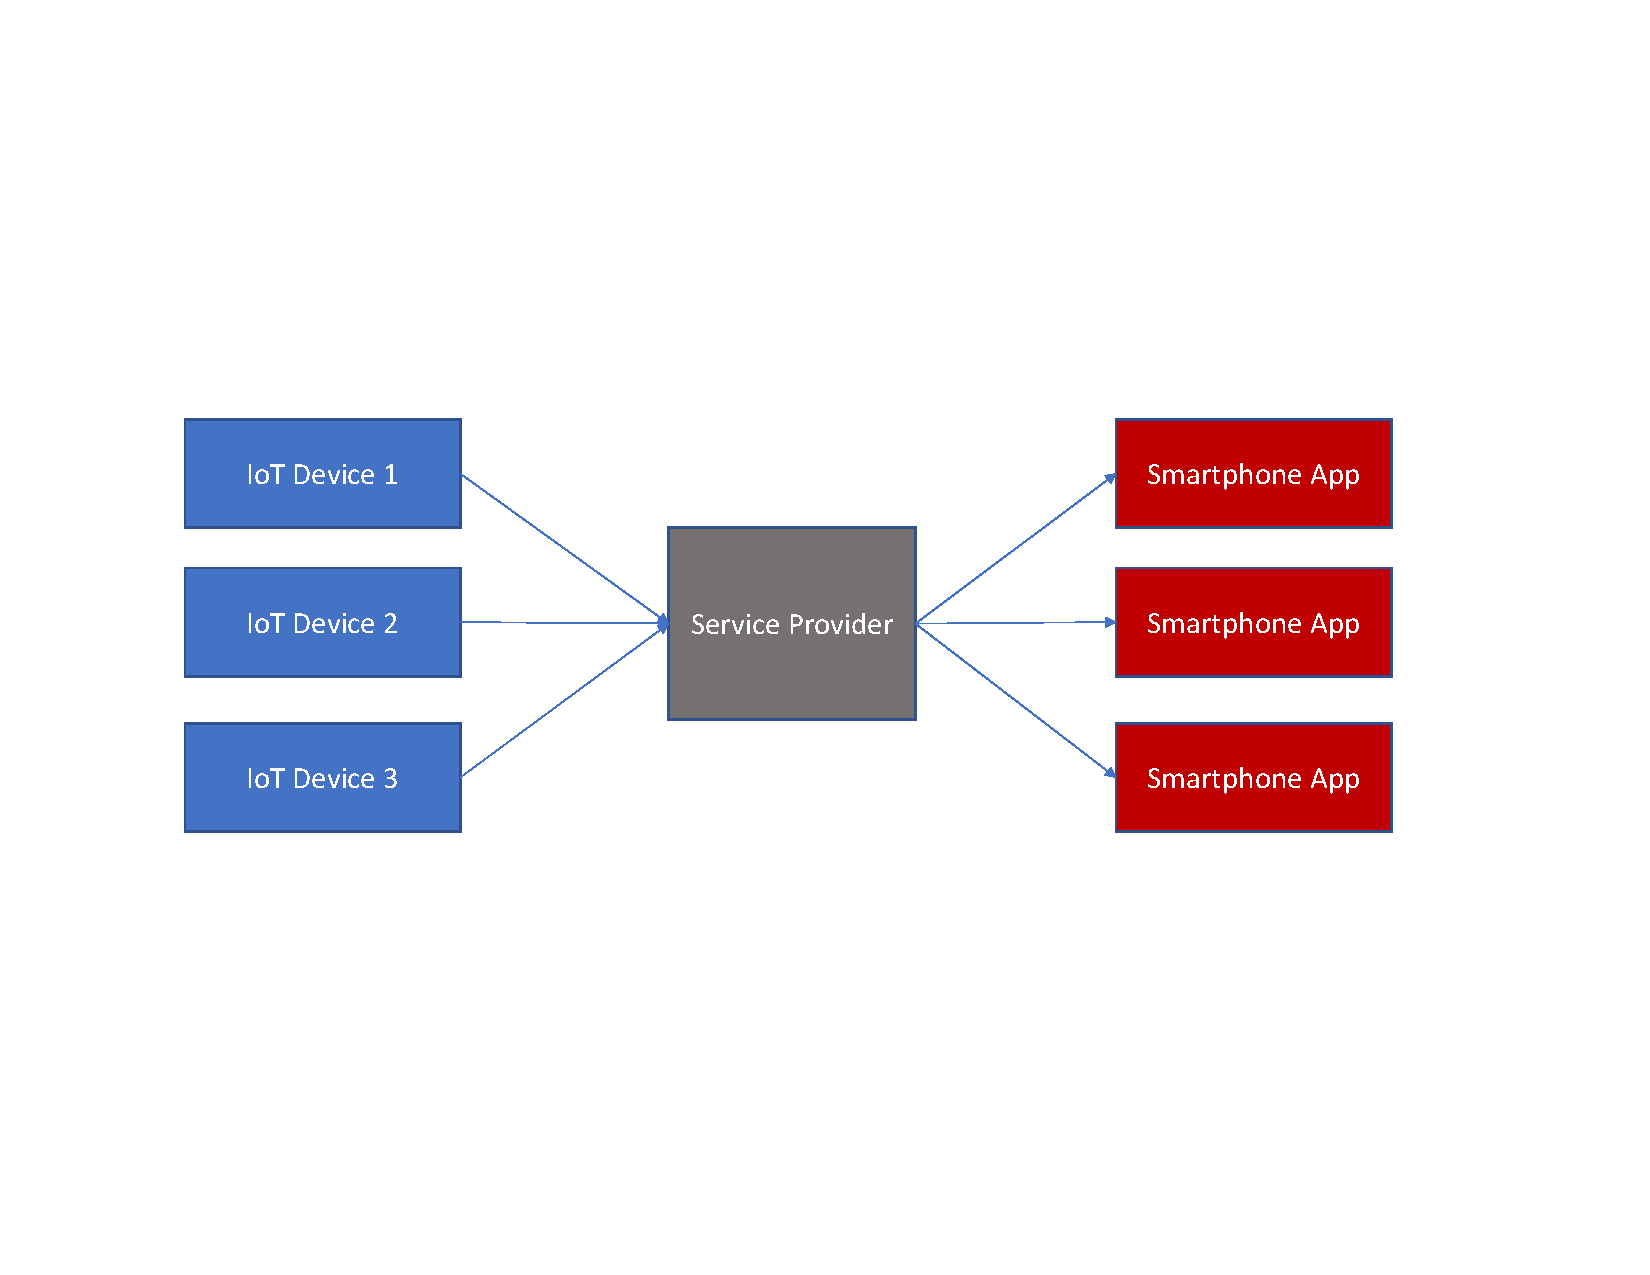
\includegraphics[width=\linewidth]{centralized_structure.pdf}
	\caption{}
	\label{fig:centralized}
\end{figure}

\section{Motivation: the need for a privacy-preserving framework}
However, connecting home appliances to the Internet introduces vulnerabilities to malicious attacks. An attacker may obtain private information, such as the user's geographic info, preference, or payment information. Attackers may even take over the control of such appliances and use them for further malicious attacks into other systems in the home network. 

\subsection{Privacy threats of IoT devices}
In reality, there have been many severe security and privacy incidents with commercial IoT devices.

In 2016, a large DDoS attack was launched on service provider Dyn using the Mirai Botnet \cite{antonakakis2017understanding}, which brought down sites including Twitter, the Guardian, Netflix and many more \cite{2006mirai}. Devices, including digital cameras and DVR players, were attacked and infected with malware. In early 2017, the FDA confirmed that St. Jude Medical's implantable cardiac devices have vulnerabilities that allow hackers to read the data and even take over the device \cite{2017fda}. In late 2019, the Ring doorbell had suffered from a data leak, exposing essential user data, including emails, passwords, time zones, and names given to specific devices \cite{2019ring}.

There already exists a rich literature that examines the security and privacy properties of these devices \cite{acar2016sok} \cite{hilt2019internet} \cite{shumailov2019hearing} \cite{apthorpe2017smart}. As we describe in the next chapter, IoT systems' security and privacy properties of have been studied widely.


\subsection{Challenges}

There are a few challenges for privacy-preserving settings on home IoT devices. 

\begin{itemize}
	\item Push notifications. While being an essential part of IoT services, push notifications are the first obstacle to building a privacy-preserving framework. Ideally, a privacy-preserving system would like to avoid any point of centralization, and so does the push notification part. However, it is hard to keep all valuable functions while achieving complete decentralization on modern mobile systems. As we described later in the discussion section, one would have to either adapt an existing commercial service or implement her own system with fewer data and energy efficiency.
	\item Limited computational power. Home IoT devices are usually built in small-size and do not have high computational power as traditional computing platforms such as desktop computers and cloud servers. The limited power is another difficulty building privacy-preserving systems, as the IoT devices will not be able to do heavy computations on-device.
\end{itemize}

\section{Overview of approach}

In this thesis, we take a different track, and rather than attempt to examine one aspect of IoT devices up close, we adopt a more holistic approach. We ask the question, "is it possible to create a privacy-preserving IoT device that offers the same features as commercially-available IoT devices?" Our goal is to determine the feasibility and potential performance costs of duplicating the capabilities of feature-rich IoT devices but in a privacy-preserving way.

In our approach, we use Tor (The Onion Router) for the purpose of obscuring the communication between IoT devices and end-user devices. Tor has a few excellent features for the task, which we describe later in this chapter.

\section{Scientific questions and contributions}

In answer to the above questions and challenges, this Master's thesis proposes a novel privacy-preserving framework for Internet-of-Things (IoT) devices that obscures the devices' traffic patterns and implements and an example application that uses this framework. A core goal of this work is to develop feature-rich IoT devices that offer similar features to existing (but non-privacy-preserving) IoT devices.

Besides, we conduct a case study that considers a specific type of home IoT device, namely an Internet-enabled video doorbell. The specific system includes a number of interesting features that may be challenging in privacy-preserving settings, which include but not limited to face and motion detection, video and audio communications and push notifications. We tackle the challenges and implement a feasible system based on our proposed design.


